\section{An Illustrative Example}

\begin{figure}[t]
\centering
 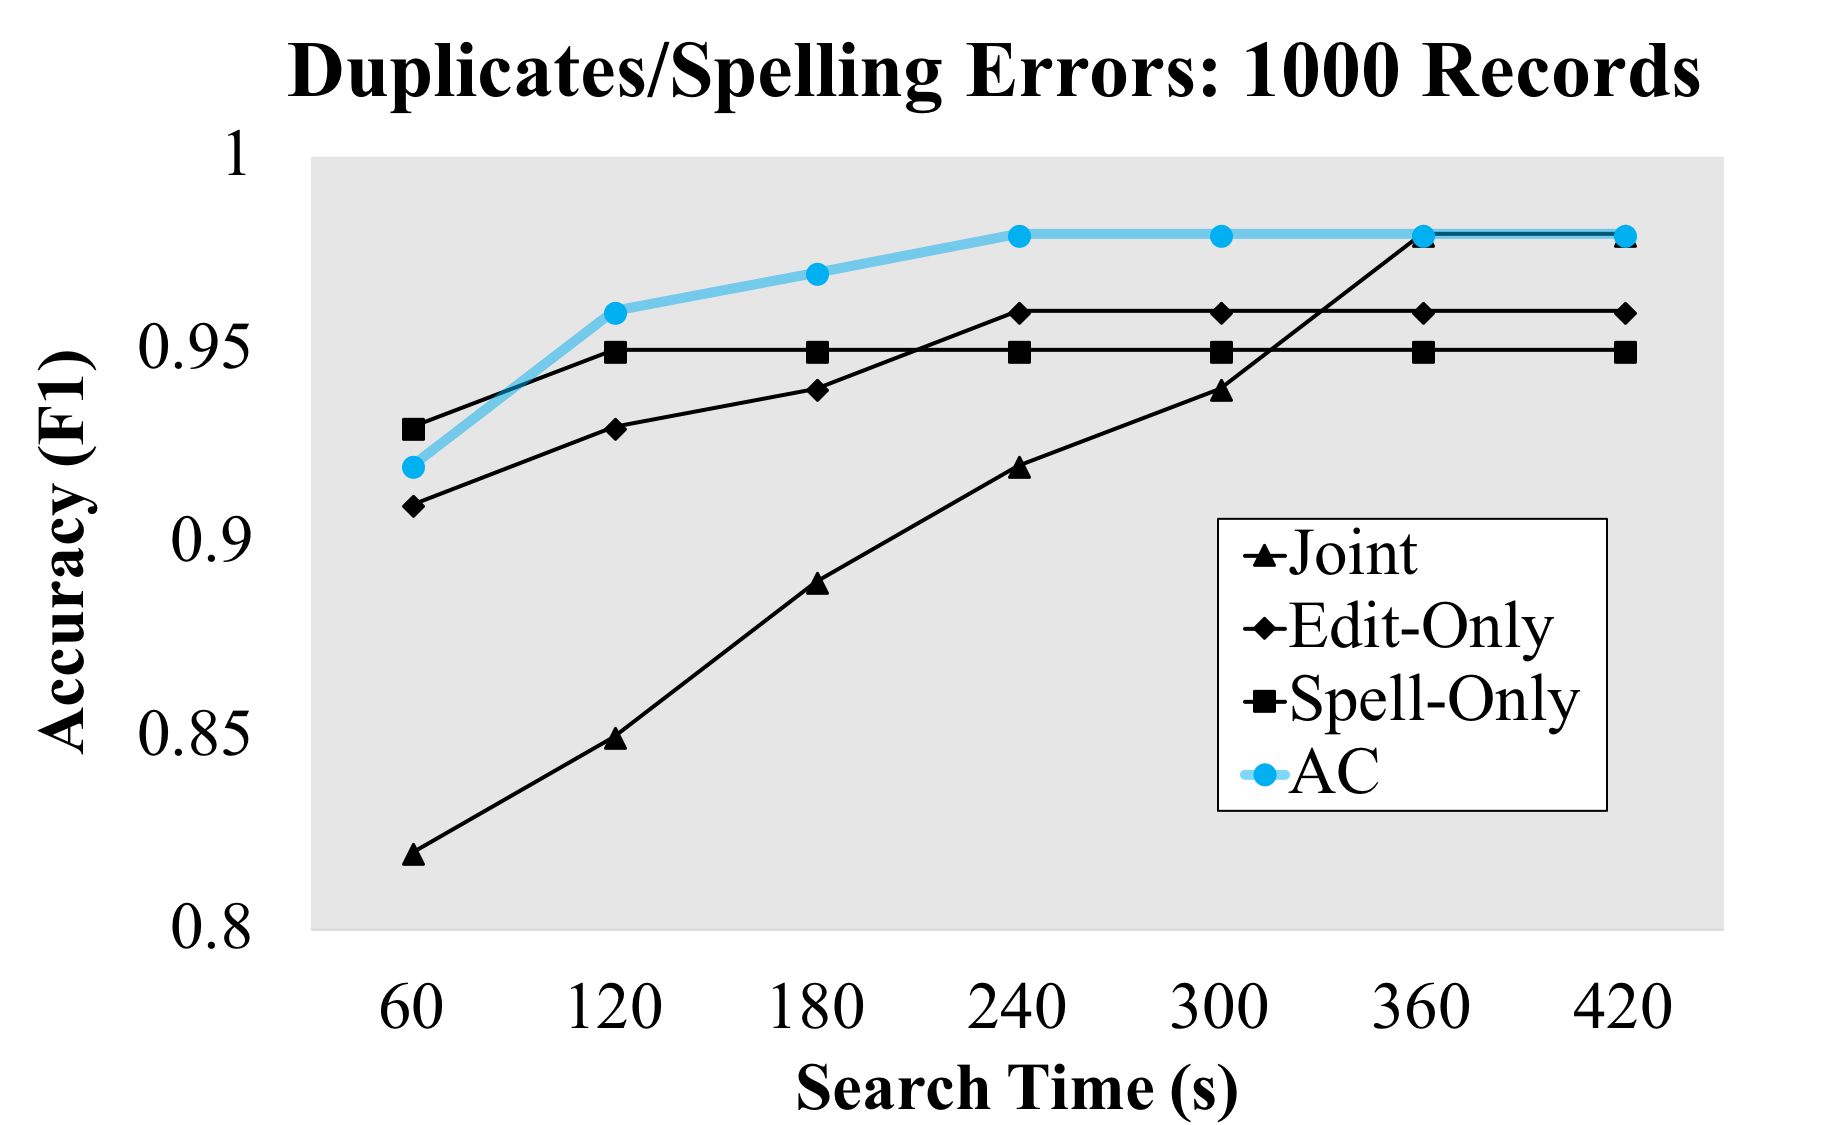
\includegraphics[width=0.9\columnwidth]{figures/teaser-experiment.png}
 \caption{\small 10\% of a dataset of dictionary words are duplicated with randomly generated spelling errors. The dataset is to be cleaned with a similarity matcher and a spell checker. Holistically, tuning the parameters of both with \textsf{python hyperopt} (BB-Full) is inefficient due to interactions between the two data cleaning options. It takes over 3x the amount of search time for the joint optimization to exceed the best tuned single cleaning method (BB-Edit and BB-SpellCheck) \label{fig:teaser}}
\end{figure}

A subtle challenge is that existing black-box search algorithms would treat the entire data cleaning pipeline as a monolithic parametrized unit.
They do not explcitly reason about interactions between pipeline components, and those effects are latently captured in the parameter space and accuracy metric.
Consider a simple experiment: we have a dataset of 1000 dictionary words (10\% of which are duplicated with randomly generated spelling errors affecting 1-3 characters), and cleaned by an edit distance similarity matcher with a tunable threshold and a spell checker with a tunable recommendation parameter.
 One would expect that jointly optimizing over the entire pipeline (cascading the matcher and spellchecker) with a black-box optimizer is more reliable than simply tuning either of the single cleaning methods. 
Figure \ref{fig:teaser} (implemented with \textsf{python hyperopt}) illustrates that this is not exactly the case, it takes over 3x the amount of search time for the joint optimization to exceed the best tuned single cleaning method.
This experiment is designed such that there is redudancy in the pipeline, where duplicates can be resolved either by spellcheck or matching.
The joint optimization method wastes evaluation cycles exploring parameter settings where both techniques significantly overlap.


In this case, we are lucky; the joint optimization converges to a reasonable solution given enough time.
However, as we scale to more complex and larger scale problems, avoiding local optima becomes a daunting challenge.
Interactions between methods may not simply be redundancies, and improperly tuned techniques might even reverse the changes made by previous steps.
We arrived at a simple architecture to address this issue by rethinking the parameter search process.
For a given parameter setting, every data cleaning method in the pipeline suggests \emph{candidate} repairs to a dataset.
These repairs are aggregated into a large set of possible transformations to apply
Then, a meta-algorithm searches over sequential compositions of the set of generated candidates.
The size of the search space can be controlled by how many parameter settings are considered and how coarse- or fine-grained the repairs are.
This process allows the system to leverage partial repairs from the pipeline when beneficial and naturally avoid problems of redundancy.

More importantly, this generate-then-search process is specialized to the idiosyncrasies of data cleaning.
Data cleaning is fundamentally a form of constraint satisfaction---easy to verify but hard to satisfy.
So, candidate generation can be much more expensive than accuracy evaluation (e.g., for Denial Constraints).
Existing search algorithms implicitly pipeline these two steps; whereas, we decouple these two steps where candidate repairs can be generated in a separate thread and the search algorithm can proceed independently.


